\documentclass{article}
\usepackage[T1]{fontenc}
\usepackage[lithuanian]{babel}
\usepackage{graphicx} % Required for inserting images
\usepackage{float} % For accuratelly placing images
\usepackage[a4paper, margin=2cm]{geometry}
\usepackage[hidelinks]{hyperref}
\usepackage{pdflscape}
\usepackage{longtable}
\usepackage{xltabular}
\usepackage{tabularx}
\usepackage{enumitem}

% For striketrghough
\usepackage{soul}

% For colored highlights 
\usepackage{xcolor}

% BEGIN: FOR SVG
% \usepackage[inkscapelatex=false]{svg}
\usepackage{svg}
\usepackage{amsmath}
% END: FOR SVG

\usepackage{everypage}
\usepackage{lscape} % Ensure landscape pages are recognized
\usepackage{lipsum}

\title{
    Įmonės „PTN“ procesų aprašymas \\
    \large versija 2.0 \\
    \large Komanda „PTN“}
\author{
    Greta Virpšaitė \\
    Rugilė Vasaitytė \\
    Domantas Keturakis \\
    Arnas Vaicekauskas \\
    \textbf{Liudas Kasperavičius (Lyderis)} 
}
\date{Spalis 2024}

\begin{document}
% Globals
\newcommand{\WorkProdIdsList}{}
\newcommand{\ProcIdsList}{}

\newcommand{\CheckUniqueWorkProd}[1]{
    \ifinlist{#1}{\WorkProdIdsList} {
    \PackageError{\WorkProdIdsList}{Work product "#1" already exists}{}
    } {
    \ifinlist{#1}{\ProcIdsList} {
        \PackageError{\ProcIdsList}{"#1" exists as a Process}{}
    } {
     \listgadd{\WorkProdIdsList}{#1}
    }
  }
}

\newcommand{\CheckUniqueProc}[1]{
    \ifinlist{#1}{\ProcIdsList} {
    \PackageError{\ProcIdsList}{Work product "#1" already exists}{}
    } {
    \ifinlist{#1}{\WorkProdIdsList} {
        \PackageError{\WorkProdIdsList}{"#1" exists as a Work product}{}
    } {
     \listgadd{\ProcIdsList}{#1}
    }
  }
}

% Work products
\newcommand{\WorkProdList}{}
\newcommand{\defineWorkProduct}[3]{%
  \expandafter\def\csname identifier#1\endcsname{#2}%
  \expandafter\def\csname name#1\endcsname{#3}%
  \CheckUniqueWorkProd{#2}
  \listgadd{\WorkProdList}{#1}
}
\newcommand{\workProdId}[1]{\textit{\csname identifier#1\endcsname}}
\newcommand{\workProdName}[1]{\csname name#1\endcsname}
\newcommand{\workProd}[1]{\workProdId{#1}. \workProdName{#1}}
\newcommand{\prodWork}[1]{\MakeLowercase{\workProdName{#1}} (\workProdId{#1})}

\newcommand{\describeWorkProd}[2]{
    \expandafter\def\csname desc#1\endcsname{#2}
}
\newcommand{\printRow}[1]{
        \workProdId{#1} &
        \workProdName{#1} &
        \csname desc#1\endcsname \\ \hline
}
\newcommand{\workProdDescriptions}{
    \forlistloop{\printRow}{\WorkProdList}
}

% Processes
\newcommand{\defineProcess}[3]{%
  \expandafter\def\csname procId#1\endcsname{#2}%
  \expandafter\def\csname procName#1\endcsname{#3}%
  \CheckUniqueProc{#2}
  \listgadd{\ProcList}{#1}
}
\newcommand{\processId}[1]{\textit{\csname procId#1\endcsname}}
\newcommand{\processName}[1]{\csname procName#1\endcsname}
\newcommand{\process}[1]{\processId{#1}. \processName{#1}}


\maketitle

\newpage
\tableofcontents


\defineWorkProduct{ClientNeeds}{KP}{Kliento poreikiai projektui}
\defineWorkProduct{ResourceEstimates}{IS}{Laiko, kainos ir žmogiškųjų išteklių sąmata}
\defineWorkProduct{FunReq}{FR}{Funkciniai reikalavimai}
\defineWorkProduct{NonFunReq}{NFR}{Nefunkciniai reikalavimai}
\defineWorkProduct{HighLevelArch}{ALSA}{Aukšto lygio sistemos architektūra}
\defineWorkProduct{Experience}{PAT}{Departamento patirtis su projektais}
\defineWorkProduct{ProjectScope}{PA}{Projekto apimtis}
\defineWorkProduct{Manual}{PNI}{Produkto naudojimo instrukcija}
\defineWorkProduct{Warranty}{GAS}{Garantinio aptarnavimo sutartis}
\defineWorkProduct{Ticket}{UK}{Užregistruota klaida}
\defineWorkProduct{Product}{PROD}{Produktas}  
\defineWorkProduct{Contract}{KS}{Sutartis su klientu} 
\defineWorkProduct{Backlog}{PUS}{Projekto užduočių sąrašas}

% SCRUM

\defineWorkProduct{SprintBacklog}{SUS}{Sprinto užduočių sąrašas}
\defineWorkProduct{SprintReviewDoc}{SPA}{Sprinto peržiūros ataskaita}
\defineWorkProduct{StoryPointRange}{PVI}{Pasakojimo vienetų intervalas}

\defineWorkProduct{Codebase}{PK}{Programinis kodas}
\defineWorkProduct{TechDoc}{TD}{Techninė dokumentacija}
\defineWorkProduct{DefectReport}{KA}{Klaidų aprašas}

\defineWorkProduct{Feedback}{GRR}{Grįžtamojo ryšio registras}

% ---------------- Define Processes

\defineProcess{EngageClient}{KĮ}{Kliento įtraukimas}
\defineProcess{RA}{RA}{Reikalavimų analizė}
\defineProcess{DraftBacklog}{UR}{Užduočių sąrašo rengimas}

\defineProcess{CreateManual}{ND}{Naudojimo dokumentacija}
\defineProcess{CloseProject}{PU}{Projekto užbaigimas}
\defineProcess{BugFix}{KT}{Klaidos taisymas}

 % Vertimus paėmiau iš čia:
 % - https://agile.lt/agile-lietuviskai-senas/
 % - https://scrumguides.org/docs/scrumguide/v1/Scrum-Guide-LTU.pdf
\defineProcess{ScrumCycle}{SC}{Scrum ciklas}
\defineProcess{Refinement}{SP}{Sprinto planavimas}
\defineProcess{Development}{ĮG}{Įgyvendinimas}
\defineProcess{Testing}{TE}{Testavimas}
\defineProcess{PartialDelivery}{PAS}{Pristatymas ir grįžtamojo ryšio surinkimas} % TODO: translate
\defineProcess{Control}{KO}{Kontrolė} % Čia gal review'iu???
 


% -----------------------Process Table Environment
\newenvironment{processTable}[1]
{
\newcommand{\tikslas}[1]{\gdef\purpose{##1}}
\newcommand{\inputs}[1]{\gdef\usedWorkProducts{##1}}
\newcommand{\outputs}[1]{\gdef\producedWorkProducts{##1}}
\newcommand{\veiklos}[1]{\gdef\activities{##1}}
\def\purpose{}
\def\usedWorkProducts{}
\def\producedWorkProducts{}
\def\activities{}
\def\processPK{#1}
}
{
\begin{tabular}{p{0.1\textwidth}|p{0.9\textwidth}}

\textbf{\processId{\processPK}} & \textbf{\processName{\processPK}} 
\\ \hline
Tikslas & \purpose 
\\ \hline
Panaudoti darbo produktai & \begin{itemize} \usedWorkProducts \end{itemize}
\\ \hline
Sukurti darbo produktai  & \begin{itemize} \producedWorkProducts \end{itemize} 
\\ \hline
Veiklos & \begin{enumerate} \activities \end{enumerate}
\label{processTable:\processPK}
\end{tabular}
}

% \begin{processTable}{PrimaryKey}
%     \tikslas{}
%     \inputs{
%        \item \workProd{Kazkas}
%     }
%     \outputs{
%        \item \workProd{Kazkas}
%     }
%     \veiklos{
%         \item Kazkokia veikla
%     }
% \end{processTable}
\section{Įmonės aprašymas}

\subsection{Įmonės pavadinimas}
„PTN“

% \subsection{"PTN" departments}

% \begin{enumerate}
%     \item  IT division
% \end{enumerate}

\subsection{Įmonės aprašymas}

% \textbf{NOTE:} Reikia aprašyti TIK IT depertamentą \newline

„PTN“ yra projektinė įmonė. „Produktų vystymas“ yra įmonės „PTN“ departamentas, kuris užsiima e.komercijos sistemų kūrimu klientams. „Produktų vystymo“ departamente įdarbinti apie 30 darbuotojų, t.\,y. šis skaičius gali šiek tiek svyruoti. Departamentas yra išskirstytas į tris komandas po maždaug 10 darbuotojų. Kiekviena komanda paraleliai dirba prie skirtingų projektų.

\subsection{Organizacinė struktūra}
Šiame dokumente modeliuojama „Produktų vystymo“ departamento komandų veikla.
\begin{table}[h!]
\centering
\begin{tabular}{p{0.1\textwidth}|p{0.9\textwidth}}
\hline
\textbf{Rolės} & \textbf{Atsakomybės} \\ \hline


% product developement & 

Projektų vadovas &

% \st{Manages and supervises the project, including setting project goals, timelines, and budgets. The project manager ensures that the development team meets deadlines and that the project is delivered successfully within the agreed-upon scope. They also act as the main point of communication between the client and the development team.}

Valdo ir prižiūri projektą, dalyvauja nustatant projekto tikslus, terminus ir biudžetą. Projekto vadovas užtikrina, kad programinės įrangos kūrimo  komanda laikytųsi terminų ir kad projektas būtų sėkmingai įgyvendintas sutarta apimtimi. Projektų vadovas komunikuoja su suinteresuotomis šalimis (SŠ).
\\ \hline
 % Deployment & Integrate developed systems with existing client platforms, for example: inventory or payment gateways. Maintain the internal IT infrastructure of the client companies. \\ \hline
Programinės įrangos kūrėjas &

% \st{ Responsible for developing the custom e-commerce software in line with the project's specifications. They ensure the functionality of the system through testing and work closely with the project manager to make sure client requirements are met. Developers also address all issues or bugs that arise during the development process. }

Atsakingas už programinės įrangos kūrimą pagal projekto tikslus.
\\ \hline

Testuotojas &

% \st{Responsible for evaluating the functionality and quality of software. They conduct various types of testing to identify defects before the product is delivered and work closely with developers to validate fixes to their reported defects. }

Atsakingas už programinės įrangos kokybės įvertinimą. Testuotojas atlieka įvairių tipų testavimą, kad nustatytų defektus prieš pristatant produktą klientui ir glaudžiai bendradarbiauja su programinės įrangos kūrėjais, kad patvirtintų praneštų klaidų pataisas.
\\ \hline

Architektas &

% \st{Designs the overall structure of the e-commerce software. The architect collaborates with developers to guide implementation and resolve complex technical challenges. }

Dalyvauja kuriant programinės įrangos architektūrą. Architektas bendradarbiauja su programinės
įrangos kūrėjais, kai kuriama programinė įranga ir padeda išspręsti sudėtingus techninius iššūkius.
\\ \hline
Analitikas & 

% \st{Gather and analyse client requirements to ensure the project meets business needs.}
Dalyvauja renkant ir analizuojant SŠ poreikius, juos dokumentuoja.
\\ \hline

% Paminėti, kad garantiniai atvejai

\end{tabular}
%\caption{Organizational Structure}
%\label{table:organizational_structure}
\end{table}


% \subsection{IT division}

% The IT department employs around 30 people. It carries out projects for private and public organisations and develops and maintains web applications in various fields.

% Short department description

% Project-based organisational structure

% E-commerce

% Agile/SCRUM

% Develops products and transfers them to the customer

% \subsubsection{Additional information}

% \paragraph{Organisational structure}
% \paragraph{Technologies used}
% \paragraph{Methodologies}




% svg debiliškai gaunas, sueis screeshot'as for the moment
% redaguoti galima čia https://demo.bpmn.io/s/start
% originalus failas: processes.bpmn

\begin{landscape}
\section{Procesų aprašymas}
Dokumente pateiktos diagramos sumodeliuotos naudojant BPMN 2.0 notaciją.
\thispagestyle{empty}
\begin{figure}[H]%[htpb!]
    \centering
    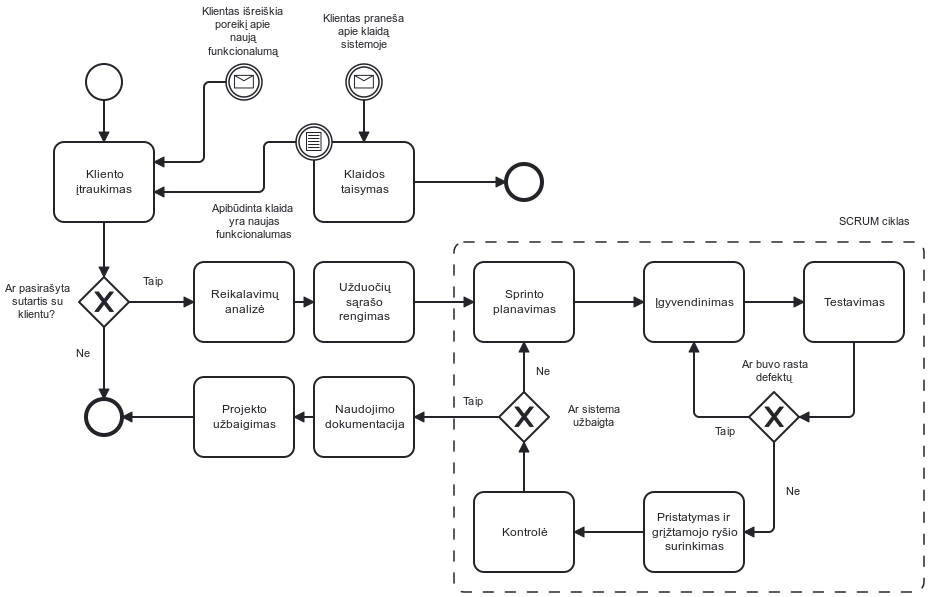
\includegraphics[width=0.85\linewidth]{task-1/etc/diagrams/processes.png}
\end{figure}
\end{landscape}

\subsection{\process{EngageClient}} % ARNAS

\begin{figure}[H]%[htpb!]
    \centering
    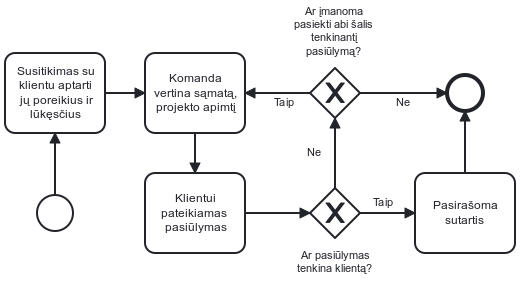
\includegraphics[width=0.75\linewidth]{task-1/etc/diagrams/engage-client.png}
\end{figure}

\begin{processTable}{EngageClient}
    \tikslas{Siekiama įvertinti kliento poreikius, rasti kompromisą dėl projekto sąmatos bei apimties ir pasirašyti sutartį.}
    \inputs{

        \item \workProd{ClientNeeds} (šis darbo produktas yra išorinis)
        
        \item \workProd{Experience}
    }
    \outputs{   
        \item \workProd{ResourceEstimates}
        
        \item \workProd{ProjectScope}
        
        \item \workProd{Contract}
    }
    \veiklos{
         \item Projektų vadovas, architektas ir analitikas bendrauja su klientu, aiškinasi jo poreikius projektui (\workProdId{ClientNeeds}). Ši veikla tęsiasi tol, kol įmonės atstovai surenka pakankamai informacijos paruošti klientui pasiūlymą.
    
        \item Projektų vadovas, architektas ir analitikas tarpusavyje įvertina kliento poreikius projektui (\workProdId{ClientNeeds}) atsižvelgdami į departamento patirtį su kitais projektais (\workProdId{Experience}) ir nustato laiko, kainos ir žmogiškųjų ištekliu sąmata (\workProdId{ResourceEstimates}) bei projekto apimtį (\workProdId{ProjectScope}). Laikas, kaina (nustatyti iš \workProdId{ResourceEstimates}), projekto apimtis (\workProdId{ProjectScope}), produkto perdavimo sąlygos ir adaptacinio laikotarpio terminas tuomet yra teisiškai įforminami sutartyje (\workProdId{Contract}). \label{activity:prepare-deal}

        \item Klientui yra pateikiama sutartis (\workProdId{Contract}). Jei klientas yra patenkintas sutarties sąlygomis, pereinama prie sutarties pasirašymo \ref{activity:sign}. Klientas gali nesutikti su sutarties sąlygomis. Tokiu atveju vyksta derybos - klientas pateikia naujus poreikius (\workProdId{ClientNeeds}) ir dar kartą vykdoma veikla \ref{activity:prepare-deal}. Jei abi šalys nesugeba rasti kompromiso, procesas gali būti nutrauktas ir darbas su klientu netęsiamas.

        \item Pasirašoma sutartis su klientu (\workProdId{Contract}). \label{activity:sign}
    }
\end{processTable}

\newpage
\subsection{\process{RA}} % DOMANTAS

\begin{processTable}{RA}
    \tikslas{
    Išskirti funkcinius ir nefunkcinius reikalavimus, apibrėžti aukšto lygio architektūrą.
    }
    \inputs{
        \item \workProd{ProjectScope}
        \item \workProd{Contract}
    }
    \outputs{
        \item \workProd{FunReq}
        \item \workProd{NonFunReq}
        \item \workProd{HighLevelArch}
    }
    \veiklos{
        \item Analitikas renka informaciją iš kliento. Pagal tai modeliuoja verslo procesus ir identifikuoja konkrečius naudotojų poreikius.
        \item Architektas ir analitikas apibrėžia funkcinius (\workProdId{FunReq}) ir nefunkcinius reikalavimus (\workProdId{NonFunReq}) iš
            \begin{itemize}
                \item identifikuotų naudotojų poreikių
                \item modeliuojamų verslo procesų
                \item projekto apimties (\workProdId{ProjectScope})
            \end{itemize}
        \item Architektas sukuria aukšto lygio sistemos architektūrą (\workProdId{HighLevelArch}) atsižvelgdamas į apibrėžtus funkcinius (\workProdId{FunReq}) ir nefunkcinius reikalavimus (\workProdId{NonFunReq}).
    }
\end{processTable}

\newpage
\subsection{\process{DraftBacklog}} % ARNAS

\begin{processTable}{DraftBacklog}
    \tikslas{Iš reikalavimų analizės rezultatų sudaryti projekto užduočių sąrašą.}
    
    \inputs{
        \item \workProd{FunReq}
        \item \workProd{NonFunReq}
        \item \workProd{HighLevelArch}
    }
    
    \outputs{
        \item \workProd{Backlog}
    }
    
    \veiklos{

        \item Architektas kartu su analitiku grupuoja susijusius funkcinius (\workProdId{FunReq}) ir nefunkcinius (\workProdId{NonFunReq}) reikalavimus bei skaido aukšto lygio architektūrą (\workProdId{HighLevelArch}) į panaudos atvejus arba bendro pobūdžio užduotis, kurios bendrai sudaro projekto užduočių sąrašą (\workProdId{Backlog}).

        \item Architektas kartu su analitiku detaliai aprašo užduotis, nurodydami kokie funkciniai (\workProdId{FunReq}) bei nefunkciniai (\workProdId{NonFunReq}) reikalavimai įeiną į konkrečios užduoties apimtį.
        \item Architektas kartu su analitiku nurodo užduočių priėmimo kriterijus, kuriais vadovaujantis galima  objektyviai įvertini ar užduotis yra įgyvendinta.
        \item Projektų vadovas, architektas ir analitikas prioritetizuoja projekto užduočių sąrašą (\workProdId{Backlog}) jį surūšiuodami.
    }
\end{processTable}

\newpage
\subsection{\process{ScrumCycle}}

%  ## Domanto klausimai
% 
%  - Jeigu sprinto backlog'e įdedamos klaidos (t.y. klaida yra tiesiog dar vienas task'as sprinto užduočių sąraše), kam tada reikalingas "KL. Klaidos" darbo produktas?

\subsubsection{\process{Refinement}}

\begin{processTable}{Refinement}
    \tikslas{
        Sudaryti sprinto užduočių sąrašą.
    }
    \inputs{
        \item \workProd{Backlog}
        \item \workProd{SprintReviewDoc} (tik nuo antro sprinto)
        \item \workProd{StoryPointRange} (tik nuo antro sprinto)
    }
    \outputs{
        \item \workProd{SprintBacklog}
        \item \workProd{Backlog}
    }
    \veiklos{
        \item Projektų vadovas, kuris atsižvelgia į sprinto peržiūros ataskaitą (\workProdId{SprintReviewDoc}), nustato sprinto tikslus. Jei istoriniai praėjusių sprintų duomenys dar neegzistuoja, nes vykdomas pirmasis sprintas, atsižvelgiama į projektų užduočių sąrašo (\workProdId{Backlog}) pirminę prioritetizacija.
        \label{SP:1}

        \item Projektų vadovas, bendro komandos susitikimo metu, \ref{SP:1}  veikloje įvardintus tikslus paskelbia komandai. Į tai atsižvelgę komandos nariai gali atnaujinti projekto užduočių sąrašo (\workProdId{Backlog}) prioritetus.
        \item Jei komandos nariai nusprendžia, kad tam tikra užduotis iš projekto užduočių sąrašo (\workProdId{Backlog})  turi būti išskaidoma į atomiškas užduotis, tai ir yra atliekama - skaidomai užduočiai sukuriamos vaikinės užduotys.
        \item Komanda kiekvienai neįvertintai užduočiai įvertina laiką ir pastangas, naudojant pasakojimo vienetus, įprastai sekančius Fibonači seką.  Tai atliekama remiantis kelių komandos narių darbine patirtimi ir bendru susitarimu. Tuomet projekto užduočių sąraše (\workProdId{Backlog}) esančios užduoties atributas -- pasakojimo vienetai -- keičiamas į nutartą skaičių.
        \item Projektų vadovas sukuria sprinto užduočių sarašą (\workProdId{SprintBacklog}) atrinkdamas aukščiausio prioriteto  užduotis iš projekto užduočių sąrašo (\workProdId{Backlog})  taip, kad jų bendra pasakojimo vienetų suma tilptų į pasakojimo vienetų intervalą (\workProdId{StoryPointRange}). Pirmojo sprinto metu, dar neturint pasakojimo vienetų intervalo, parenkama tiek užduočių, kiek komanda bendru nutarimu nusprendžia.
        \item Komandos nariai planuoja, kas atliks kurią sprinto užduotį. Nutarus, sprinto užduočių sąraše (\workProdId{SprintBacklog}) kiekvienos užduoties atributas -- atsakingas asmuo --  keičiamas į už užduoties įgyvendinimą atsakingo asmens vardą ir pavardę.
    }
\end{processTable}

\newpage
\subsubsection{\process{Development}}

\begin{processTable}{Development}
    \tikslas{
         Atlikti sprinto užduočių sąraše išvardytas užduotis.
    }
    \inputs{
        \item \workProd{SprintBacklog}
        \item \workProd{DefectReport}
        \item \workProd{Codebase}
        \item \workProd{TechDoc}
    }
    \outputs{
        \item \workProd{SprintBacklog}
        \item \workProd{Codebase}
        \item \workProd{TechDoc}
    }
    \veiklos{
        \item Kai programinės įrangos kūrėjai atlieka jiems priskirtą užduotį, užduoties statusas keičiamas IN PROGRESS. 
        \item Jei šis procesas vykdomas, kai užduotis buvo grąžinta į įgyvendinimą (\textit{ĮG}) po testavimo proceso (\textit{TE}), programinės įrangos kūrėjai atsižvelgia į klaidų aprašus (\workProdId{DefectReport}), kad ištaisytų klaidas. Kitu atveju veikla praleidžiama.
        \label{IG:2}
        \item Kiekvienas programinės įrangos kūrėjas rašo kodą, taip papildydami programinį kodą   
        (\workProdId{Codebase}). 
        \label{IG:3}
        \item Programinės įrangos kūrėjai rašo vienetų testus, kurie padengia 70\% kodo eilučių, kad užtikrintų kodo korektiškumą. Laikoma, kad yra atnaujinamas programinis kodas (\workProdId{Codebase}).
        \label{IG:4}
        \item Programinės įrangos kūrėjas, atsakingas už užduotį, keičia užduoties statuso atributą į \mbox{IN~REVIEW}.
        \label{IG:5}
        \item Užduotį, kuri yra IN REVIEW, kitas komandos narys peržiūri, komentuoja kodą. Jeigu kitas komandos narys pareikalauja pakeitimų, pakeičia užduoties statusą į IN PROGRESS. Už užduotį atsakingas asmuo turi pakartoti \ref{IG:3}-\ref{IG:6} veiklas.
        \label{IG:6}
        \item Kitam komandos nariui patvirtinus kodo kokybę, programinės įrangos kūrėjas pažymi, kad programinį kodą (\workProdId{Codebase}) galima testuoti - užduoties statusas keičiamas į TESTING, o atributas atsakingas asmuo  keičiamas į už užduoties testavimą atsakingo asmens vardą ir pavardę.  
        \label{IG:7}
        \item Visą reikalingą techninę dokumentaciją (\workProdId{TechDoc}) parašo programinės įrangos kūrėjas.
        \label{IG:8}
        \item Laikas, praleistas atliekant \ref{IG:2}-\ref{IG:8} veiklas pažymimas sprinto užduočių sąrašo (\workProdId{SprintBacklog})  užduoties atribute  „kūrimo valandos“.
    }
\end{processTable}

\newpage
\subsubsection{\process{Testing}}

\begin{processTable}{Testing}
    \tikslas{
        Verifikuoti programinį kodą.
    }
    \inputs{
        \item \workProd{SprintBacklog}
        \item \workProd{DefectReport} (nuo antro sprinto)
        \item \workProd{Codebase}
        \item \workProd{TechDoc}
    }
    \outputs{
        \item \workProd{DefectReport}
        \item \workProd{SprintBacklog}
        \item \workProd{Codebase}
    }
    \veiklos{
        \item Kiekvienas testuotojas atlieka jam priskirtą užduotį kaip nurodyta sprinto užduočių saraše (\workProdId{SprintBacklog}). 
        \label{TE:1}
        \item Testuotojai testuoja užduoties programinį kodą (\workProdId{Codebase}) pagal užduoties aprašymą, kuriame nurodyti funkciniai ir nefunkciniai reikalavimai. Jie taip pat atsižvelgia į užduoties priėmimo kriterijus, kurie nurodyti viename iš užduoties atributų. Pagal patirtį arba pasitarę su kitais komandos nariais, testuotojai gali nuspręsti atlikti integracijos, našumo, saugumo, regresijos ir kitus testus. 
        \label{TE:2}
        \item Testuotojai rašo arba taiso klaidų aprašus (\workProdId{DefectReport}), kad jie atspindėtų programinio kodo kokybės būklę.
         \label{TE:3}
        \item Jei šio proceso metu buvo rasta klaidų, užduotis grąžinama atgal į įgyvendinimo (\processId{Development}) procesą, kad programinės įrangos kūrėjai išspręstų klaidas. Testuotojas turi pakeisti užduoties būseną, kad sprinto užduočių sąraše (\workProdId{SprintBacklog}) būtų nurodyta, kad jos statusas IN PROGRESS, o atributas -- atsakingas asmuo -- keičiamas į už užduoties taisymą atsakingo asmens vardą ir pavardę.  
         \label{TE:4}
        \item Laikas, kuris buvo praleistas atliekant \ref{TE:2}-\ref{TE:4} veiklas pažymimas sprinto užduočių sąraše (\workProdId{SprintBacklog}) esančios užduoties atribute 
         „testavimo valandos“.
    }
\end{processTable}

\newpage
\subsubsection{\process{PartialDelivery}}

\begin{processTable}{PartialDelivery}
    \tikslas{
       Pristatyti suinteresuotoms šalims atliktą darbą ir surinkti grįžtamąjį ryšį.
    }

    \inputs{
        \item \workProd{Codebase}
        \item \workProd{Backlog}
    }
    \outputs{
       \item \workProd{Feedback}
       \item \workProd{Product}
    }
    \veiklos{
        \item Programinės įrangos kurėjai sukuria naujos produkto versijos (\workProdId{Product}) artefaktą.
        \item Programinės įrangos kūrėjas pristato produktą (\workProdId{Product}) suinteresuotoms šalims.
        \item Komandos nariai išklauso SŠ atsiliepimus apie atliktą darbą. Aptaria visus trūkumus, galimus patobulinimus ir pakeitimus projekto užduočių saraše (\workProdId{Backlog}).
        \item Projekto vadovas surašo surinktus atisiliepimus į grįžtamojo ryšio registrą (\workProdId{Feedback}).
    }
\end{processTable}

\newpage
\subsubsection{\process{Control}}

\begin{processTable}{Control}
    \tikslas{
        Įvertinti kaip sekėsi sprintas ir suderinti būsimų scrum ciklų patobulinimus.
    }
    \inputs{
        \item \workProd{DefectReport}
        \item \workProd{SprintBacklog}
        \item \workProd{ResourceEstimates}
        \item \workProd{StoryPointRange}
        \item \workProd{Feedback}
        \item \workProd{Backlog}
    }
    \outputs{
        \item \workProd{SprintReviewDoc}
        \item \workProd{StoryPointRange}
    }
    \veiklos{
        \item Visi komandos nariai apmąsto sprinto eigą, aptaria, kas pavyko ir su kokiais sunkumais susidūrė. Visi komandos nariai surašo savo  atsiliepimus.
        
        \item Projekto vadovas peržiūri sprinto užduočių sąrašą (\workProdId{SprintBacklog}), palygina faktinį užduotims atlikti sugaištą laiką su kūrimo valandų įvertinimais ir parengia laiko valdymo ataskaitą atsižvelgdamas į likusį laiką iš pradinių sąmatų (\workProdId{ResourceEstimates}).

        \item Remiantis grįžtamojo ryšio registru (\workProdId{Feedback}) ir laiko valdymo ataskaita, projekto vadovas atlieka projekto užduočių sąrašo (\workProdId{Backlog}) atnaujinimą, prireikus, užduočių prioritetų keitimą, pasakojimo vienetų intervalo (\workProdId{StoryPointRange}) patikslinimą. Šie pakeitimai fiksuojami sprinto peržiūros ataskaitoje (\workProdId{SprintReviewDoc}).
        
        \item Remiantis komandos atsiliepimais, komanda ir projektų vadovas nustato komandos procesų pakeitimus, kurie įsigalioja nuo kito sprinto.
        % \item Based on \textbf{1-2} and feedback documentation (\textit{FD}), the project manager and scrum team identifies necessary adjustments for the next sprint.
        
        % NOTE: Bet ar tai tikrai reikia čia atlikti? Gal geriau tai pažymėti sprinto peržiūros ataskaitoj ir td koregavimas atliekamas Sprinto Planavime?? also jeigu keičiama čia, tai reikia pridėti atitinkamai prie input'ų ir output'ų.
        
        % This includes updating the project backlog (\textit{PB}), reprioritizing tasks as needed and capturing these changes in the sprint review report (\textit{SRR}), refining the story point range (\textit{SP}).

        \item Jei projekto užduočių sąraše (\workProdId{Backlog}) visų užduočių statusas yra DONE, pereinama prie naudojimo dokumentacijos (\processId{CreateManual}), o SCRUM ciklai šiam projektui nebetęsiami.
        % NOTE: čia gal nurodyti kokiomis sąlygomis nebereikia kitų sprint'ų?
        % \item The project manager closes project if necessary - if no further sprints are required, they transition to usage documentation.
    }
\end{processTable}

\newpage
\subsection{\process{CreateManual}}

\begin{processTable}{CreateManual}
    \tikslas{Paruošti produkto naudojimo instrukciją, suprantamą naudotojams.}
    \inputs{
        \item \workProd{Backlog}
        \item \workProd{Product}
    }
    \outputs{
            \item \workProd{Manual}
    }
    \veiklos{
        \item Iš užduočių sąrašo (\workProdId{Backlog}) išrenkami panaudos atvejai. 
        \item Detaliai aprašomi visi žingsniai kiekvienam panaudos atvejui įgyvendinti naudojant produkto (\workProdId{Product}) iliustracijas. \label{CreateManual/1}
        \item Detaliai aprašomos visos produkto (\workProdId{Product}) funkcijos (t.\,y. kaip jomis pasinaudoti). \label{CreateManual/2}
        \item Iš \ref{CreateManual/1} ir \ref{CreateManual/2} veiklų rezultatų sudaromas struktūrizuotas, vientisas dokumentas - \prodWork{Manual}
        \item Atliekama produkto naudojimo instrukcijos (\workProdId{Manual}) validacija - paruoštas dokumentas peržiūrimas kolegų iš kitų padalinių, įsitikinama, jog instrukcija suprantama pirmą kartą produktą (\workProdId{Product}) naudojantiems žmonėms. \label{CreateManual/3}
        \item Kol netenkinamas \ref{CreateManual/3} punktas, atliekami naudojimo instrukcijos pakeitimai.
        }
\end{processTable}

\begin{figure}[!h]
    \centering
    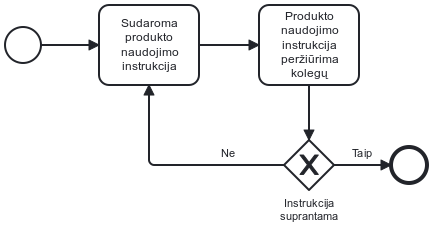
\includegraphics[width=0.75\linewidth]{task-1/etc/diagrams/Manual.png}
\end{figure}
% --------------------------------------------------------------------
\newpage
\subsection{\process{CloseProject}}
\begin{processTable}{CloseProject}
    \tikslas{Užbaigti projektą, perduoti paruoštą naudojimui produktą klientams.}
    \inputs{
        \item \workProd{Product}
    	\item \workProd{Contract}
    	\item \workProd{Backlog}
    	\item \workProd{TechDoc}
    	\item \workProd{Manual}
    }
    \outputs{
        \item \workProd{Warranty}
        \item \workProd{Experience}
    }
    \veiklos{
        \item Atliekami sutartyje (\workProdId{Contract}) numatyti produkto (\workProdId{Product}) perdavimo klientui darbai.
        \item Klientui perduodama \prodWork{Manual}.
        \item Klientui perduodama \prodWork{TechDoc}.
        \item Sudaroma ir pasirašoma \prodWork{Warranty}, kurioje numatomas garantinio aptarnavimo laikotarpis.
    	\item Atliekama vidinė komunikacija apie užbaigtą projektą. Projekto vadovas dalinasi projekto eiga, priimtais kritiniais sprendimais ir rezultatais. Taip kaupiama \prodWork{Experience}. 
    	\item Kol nesibaigia sutartyje (\workProdId{Contract}) numatytas adaptacinis laikotarpis, klientams teikiama techninė pagalba.
    }
\end{processTable}

\begin{figure}[!h]
    \centering
    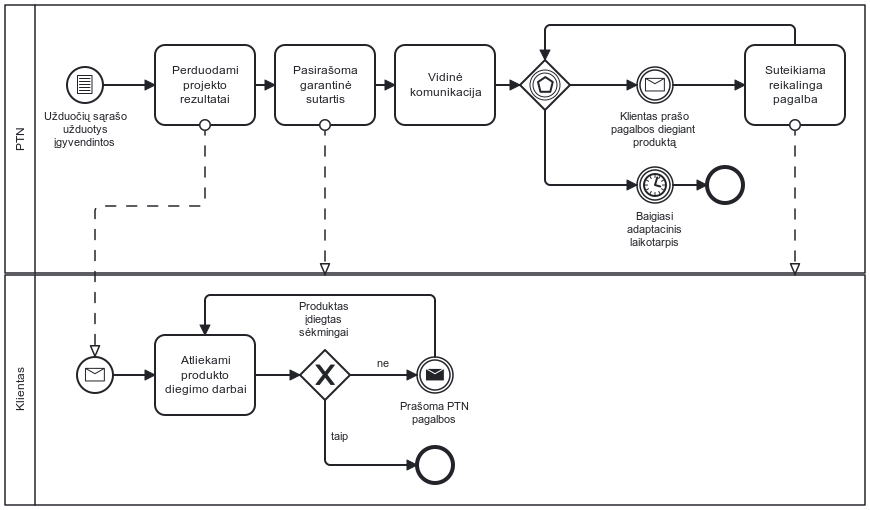
\includegraphics[width=0.8\linewidth]{task-1/etc/diagrams/projectClosure.png}
\end{figure}
\newpage

%----------------------------------------


\subsection{\process{BugFix}}
\begin{processTable}{BugFix}
    \tikslas{Ištaisyti ne dėl kliento kaltės kilusias produkto klaidas.}
    \inputs{
        \item \workProd{Product}
    	\item \workProd{TechDoc}
    	\item \workProd{Contract}
    	\item \workProd{Warranty}
    	\item \workProd{Ticket} (išorinis darbo produktas)
    	\item \workProd{Manual}
     }
    \outputs{
        \item \workProd{Ticket}
        \item \workProd{Product}
    }
    \veiklos{
        \item Atliekama pirminė užregistruotos klaidos (\workProdId{Ticket}) analizė.
	   \item Jei užregistruota klaida (\workProdId{Ticket}):
            \begin{enumerate}[label=\alph*)] 
        		\item kyla dėl produkto (\workProdId{Product}) naudojimo nesilaikant produkto naudojimo instrukcijos (\workProdId{Manual})
        		\item kyla eksploatuojant produktą (\workProdId{Product}) netinkamomis, t.\,y. neatitinkančiomis techninės dokumentacijos (\workProdId{TechDoc}), sąlygomis
        		\item yra ne klaida, o neegzistuojančio ir sutartyje (\workProdId{Contract}) nenumatyto funkcionalumo įgyvendinimo prašymas
        		\item neatitinka garantino aptarnavimo sutartyje (\workProdId{Warranty}) numatytų sąlygų
        		\item yra užregistruota po garantino aptarnavimo sutartyje (\workProdId{Warranty}) numatyto garantinio laikotarpio
            \end{enumerate}
            tuomet užregistruota klaida (\workProdId{Ticket}) nėra taisoma ir šis procesas (\processId{BugFix}) yra užbaigiamas nevykdant tolesnių veiklų.
    	\item Atliekama klaidos kilimo priežasties analizė (root cause analysis).
    	\item Kuo įmanoma greičiau ištaisoma klaida ir sukuriama nauja produkto (\workProdId{Product}) versija.
    	\item Nauja produkto (\workProdId{Product}) versija perduodama klientams.
    	\item Užregistruota klaida (\workProdId{Ticket}) „Jira“ platformoje papildoma su klaidą ištaisančia prdoukto (\workProdId{Product}) versija bei klaidos kilimo priežastimi.    
    }
\end{processTable}
\newpage

%----------------------------------------

% \begin{processTable}{PrimaryKey}
%     \tikslas{}
%     \inputs{
%        \item \workProd{Kazkas}
%     }
%     \outputs{
%        \item \workProd{Kazkas}
%     }
%     \veiklos{
%         \item Kazkokia veikla
%     }
% \end{processTable}


%----------------------------------------
\newcommand{\hiden}[1]{}

\describeWorkProd{ResourceEstimates}{
Dokumentas, kuriame surašytas projekto pabaigos terminas, projekto kaina ir informacija apie už projekto įgyvendinimą atsakingus darbuotojus. 
}

\describeWorkProd{FunReq}{

% > Software requirements express the needs and
% constraints placed on a software product that
% contribute to the solution of some real-world
% problem.

%     -- SWEBOK

% > At its most basic, a software requirement is a
% property that must be exhibited by something in order to solve some problem in the real world.

%     -- SWEBOK

% > Functional requirements describe the functions
% that the software is to execute; for example, for-
% matting some text or modulating a signal. They
% are sometimes known as capabilities or features.
% A functional requirement can also be described
% as one for which a finite set of test steps can be
% written to validate its behavior.

%     -- SWEBOK

Funkciniai reikalavimai apibūdina funkcijas, kurias turi atlikti produktas, kad būtų išspręsta kliento problema.
}

\describeWorkProd{NonFunReq}{
Nefunkciniai reikalavimai yra kokybės kriterijai, t.\,y. jie nusako, kaip produktas turi atlikti savo funkcijas. Jie apibrėžia, kokius našumo, greitaveikos\hiden{performance}, saugumo\hiden{security}, panaudojamumo\hiden{usability}, pasiekiamumo\hiden{reliability} kriterijus turi atitkti produktas.
}

\describeWorkProd{HighLevelArch}{

Nusako kaip programinė įranga yra organizuojama į atskirus komponentus, jų savybes bei kaip tie komponentai sąveikauja.

% > * Architectural design (also referred to as high-level design and top-level design) describes how software is organized into components.

%     -- SWEBOK

% > In its strict sense, a software architecture is
% “the set of structures needed to reason about
% the system, which comprise software elements,
% relations among them, and properties of both”

%     -- SWEBOK
}

\describeWorkProd{ProjectScope}{
Dokumentas, apibūdinantis, kas yra planuojama sukurti projekto metu, kokios numatytos sistemų funkcijos ir kokios funkcijos yra už kuriamų sistemų ribų.
}

\describeWorkProd{Manual}{Skirta sistemos naudotojams. Čia aprašomi visi panaudos atvejai, visos produkto funkcijos bei kaip jomis naudotis. „PTN“ įmonė užtikrina teisingą produkto veikimą, jei laikomasi šio dokumento, priešingu atveju -- „PTN“ nėra atsakinga už galimus produkto sutrikimus.
}

\describeWorkProd{Warranty}{Šis dokumentas pasirašomas perduodant klientui užbaigtą produktą. Čia numatomos sąlygos, kuriomis kliento pastebėtos produkto klaidos bus ištaisomos „PTN“ įmonės be papildomo mokesčio per tam tikrą (taip pat šiame dokumente) numatytą laiką. Ši sutartis turi numatytą galiojimo laikotarpį.
}

\describeWorkProd{Ticket}{Tai dokumentas, užregistruotas užduočių sekimo platformoje („Jira“), kuriame privalo būti ši informacija:
\begin{itemize}
    \item Registravimo data ir laikas
    \item Autorius („PTN“ įmonės darbuotojas arba kliento atstovas)
    \item Detalus klaidos aprašymas
    \item Kuo įmanoma detalesnis situacijos, kurioje įvyksta klaida, aprašymas
    \item Produkto versija, kurioje pastebėta klaida
\end{itemize}
Šio dokumento statusas atspindi klaidos taisymo proceso (\processId{BugFix}) stadiją:
\begin{itemize}
    \item OPEN -- klaida užregistruota
    \item IN REVIEW -- atliekama pirminė analizė
    \item REJECTED -- kliento pateikta klaida nebus taisoma (pridedama priežastis) 
    \item IN PROGRESS -- atliekama \textit{Root Cause Analysis} ir ruošiama nauja produkto versija
    \item DONE -- nauja produkto versija išleista ir perduota klientui
\end{itemize}
}

\describeWorkProd{Contract} {
Sutartis tarp įmonės ir kliento, kuri įpareigoja įmonę įvykdyti kliento užsakymą pagal numatytą apimtį, laiką ir biudžetą. Taip pat nurodytos produkto perdavimo sąlygos ir adaptacinis laiko terminas (perdavus produktą, suteikiama techninė pagalba tam tikrą numatytą laikotarpį).
}

\describeWorkProd{Backlog}{
Užduočių sąrašą sudaro bent viena užduotis. Užduotys gali būti kelių tipų:

\begin{itemize}

    \item Panaudos atvejis - tai stambi užduotis, kuri yra suformuluota iš sistemos naudotojo perspektyvos ir apibūdina sistemos funkcionalumą.

    \item Bendro pobūdžio užduotis - tai užduotis, kuri negali būti apibūdinta iš naudotojo perspektyvos, tačiau aprašo būtiną darbą sistemos veikimui užtikrinti.

\end{itemize}

Visi išvardinti užduočių tipai gali turėti vaikines, nedalomas užduotis. Taip pat, kiekviena užduotis turi tam tikrus atributus; ne visi yra iš karto priskiriami užduotims jas sukūrus, tačiau atributai gali keistis projekto gyvavimo laikotarpiu, jei atsirastų toks poreikis. Užduočių atributų sąrašas:

\begin{itemize}
    \item Pavadinimas - trumpas pavadinimas nusakantis užduoties kontekstą 
    \item Aprašas - išsamus tekstas aprašantis užduotį, jame atskleidžiami funkciniai ir nefunkciniai užduoties reikalavimai.
    \item Statusas - nusako kokioje stadijoje yra užduotis. Gali turėti tik viena iš šių reikšmių:
    \begin{itemize}
        \item OPEN - užduotis nepradėta. Kiekviena nauja užduotis automatiškai turi šį statusą
        \item IN PROGRESS - užduotis yra daroma
        \item IN REVIEW - užduotis padaryta ir reikalauja bent vieno komandos nario peržiūros
        \item TESTING - užduotis yra perduota testuotojams
        \item DONE - užduotis įgyvendinta
    \end{itemize}
    \item Priėmimo kriterijai - sąlygos, kurios turi būti tenkinamos norint keisti užduoties statusą į DONE
    \item Pasakojimo vienetai - skaliarinis įvertis, kuris nusako reliatyvų užduoties sudėtingumą.
    \item Atsakingas asmuo - šiuo metu užduotį atliekantis arba testuojantis asmuo.
    \item Prioritetas - užduoties svarba. Vertinama reliatyviai, t.\,y. kuo užduočių sąraše užduotis yra aukščiau, tuo užduotis turi būti greičiau atlikta.
    \item Kūrimo valandos - užduočiai įgyvendinti skiriamos valandos.
    \item Kūrimo valandų įvertinimas - užduočiai įgyvendinti planuojamas valandų kiekis.
    \item Testavimo valandos - užduočiai testuoti skiriamos valandos.
\end{itemize}

}

\describeWorkProd{SprintBacklog}{
Tai yra užduočių sąrašas, kuris yra projekto užduočių sąrašo poaibis. Jį sudaro sprintui atrinktos užduotys iš projekto užduočių sąrašo, taigi, užduoties tipai gali būti tie patys kaip ir (\workProdId{Backlog}), o užduočių atributų būsena (\workProdId{Backlog}) ir (\workProdId{SprintBacklog}) visada sutampa. 
}

\describeWorkProd{SprintReviewDoc} {
Dokumentas, kuriame fiksuojami sprinto pabaigoje vykstančio susitikimo metu aptarti komandinio darbo pakeitimai. Be to, sprinto peržiūros ataskaita apima rekomendacijas kitam sprintui, numatytus pakeitimus, atnaujintus prioritetus. Ši ataskaita padeda komandai mokytis iš ankstesnių sprintų ir tobulinti darbo procesą ateityje.
}

\describeWorkProd{StoryPointRange} {
 Tai diapazonas, kuris nurodo bendrą sprintui skirtų užduočių sudėtingumą. Šis intervalas padeda komandai nustatyti, kiek darbų jie gali atlikti per sprintą, remiantis ankstesniais sprintais arba bendra komandos patirtimi. Pasakojimo vienetai (angl. story points) dažniausiai naudojami įvertinti užduočių sudėtingumą ar darbų apimtį, atsižvelgiant į laiką, resursus ir pastangas, reikalingas užduotims atlikti.
}

\describeWorkProd{Codebase} {
Tai programinės įrangos sukurtas instrukcijų rinkinys, kuris įgyvendina produkto užduočių sąraše (\workProdId{Backlog}) nurodytus reikalavimus. Programinis kodas apima ir  programininės įrangos kūrėjų parašytus vienetų testus ir testuotojų sukurtus testus.
}

\describeWorkProd{TechDoc} {
Dokumentas, kuriame aprašoma, kokios programinės įrangos funkcijos, struktūra ir kiti techniniai aspektai. Techninę dokumentaciją rašo programinės įrangos kūrėjai, kad ji būtų naudinga tiek kitiems kūrėjams, tiek projekto komandos nariams. Dokumentacija yra svarbi norint užtikrinti aiškų supratimą apie programos sistemos veikimą bei lengvą jos palaikymą ir vystymą ateityje.
}

\describeWorkProd{DefectReport} {
Dokumentas, kuriame apibūdinamos programinės įrangos klaidos, pastebėtos testavimo metu. Tipiškai klaidų aprašymas apima šiuos elementus:

\begin{itemize}
    \item Klaidos ID – unikalus identifikatorius, skirtas kiekvienai klaidai sekti.
    \item Klaidos aprašymas – detali informacija apie tai, kas neveikia arba kurioje sistemos dalyje pastebėta problema.
    \item Žingsniai klaidai atkurti – žingsniai, kurie leidžia atkurti klaidą, siekiant patikrinti ir išspręsti problemą.
    \item Tikėtinas rezultatas – aprašymas, kaip sistema turėtų veikti normaliomis sąlygomis.
    \item Gautas rezultatas – aprašymas, kas iš tikrųjų nutiko.
    \item Svarba – nurodo, kiek svarbu yra išspręsti klaidą (kritinė, didelės svarbos, mažos svarbos).
    \item Klaidų statusas – dabartinė klaidos būsena.
    \item Atsakingas asmuo – nurodomas asmuo, kuris atsakingas už klaidos ištaisymą.
\end{itemize}
}

\describeWorkProd{Feedback} {
Dokumentas, kuriame fiksuojami suinteresuotų šalių pateikti atsiliepimai apie projekto pokyčius, siūlomus patobulinimus.
}

\describeWorkProd{Product} { 
Programų sistema, kurią vysto „Produktų vystymo“ departamentas, pagal projekto apimtį (\workProdId{ProjectScope}).
}

\describeWorkProd{Experience}{
    „Produktų vystymo“ departamento sukaupta patirtis, kuri padeda įvertinti laiko, kainos ir žmogiškųjų išteklių sąmatą (\workProdId{ResourceEstimates}) bei projekto apimtį (\workProdId{ProjectScope}).
}

\describeWorkProd{ClientNeeds}{
    Kliento lūkesčiai projektui kurie apibūdina funkcionalumą, apimtį, biudžetą ir terminus. Šie poreikiai surenkami per susitikimus su klientu ir yra svarbūs nusprendžiant projekto apimtį, sąmatą bei sutarties sudarymui.
}



% -------------- END OF DESCRIPTIONS-------------------------
\section{Darbo produktų sąrašas}

\begin{longtable}{|c|p{0.15\textwidth}|p{0.75\textwidth}|}
    \hline
    \textbf{Id} & \textbf{Pavadinimas} & \textbf{Aprašymas} \\ \hline
    \workProdDescriptions
\end{longtable}

\end{document}
